% --- INICIO DEL MÓDULO: 02_punto3.tex ---

\subsection{Caracterización del Ruido Blanco en Tiempo y Frecuencia}

Al observar la señal en el dominio del tiempo, se evidenció una forma de onda erratica y sin ningún patrón repetitivo. Los picos de voltaje varían de forma impredecible en cada instante de muestreo, lo cual comprueba físicamente que las muestras de ruido blanco son variables aleatorias descorrelacionadas e independientes entre sí.

El fenómeno más destacable se registró en el dominio de la frecuencia. Al analizar la Densidad Espectral de Potencia (PSD), la gráfica no mostró lóbulos ni campanas (como ocurre con los pulsos rectangulares), sino que exhibió una banda completamente plana y horizontal que se extiende a lo largo de todo el rango de frecuencias observable por el analizador (desde $-f_s/2$ hasta $+f_s/2$). Esta "planitud" espectral es una característica del ruido blanco, demostrando que su energía se distribuye equitativamente en todas las frecuencias del espectro evaluado.

Al realizar pruebas variando el parámetro de amplitud del ruido en el bloque generador, se observó que la forma plana de la PSD no se altera. El único efecto visible en el espectro es un desplazamiento vertical de la gráfica (un aumento en la magnitud de dB), lo que confirma que un aumento en la amplitud del ruido incrementa la potencia total inyectada al sistema de manera uniforme en todo el ancho de banda. con un cambio en la amplitud de 0.2 se evidencia que la ganancia relativa del ruido tiene su centro alrededor de -50 db mientras que con una amplitud de unidad se tiene aproximadamente el centro en -40db

\begin{figure}[htbp]
\centering
\begin{subfigure}[b]{0.45\textwidth}
    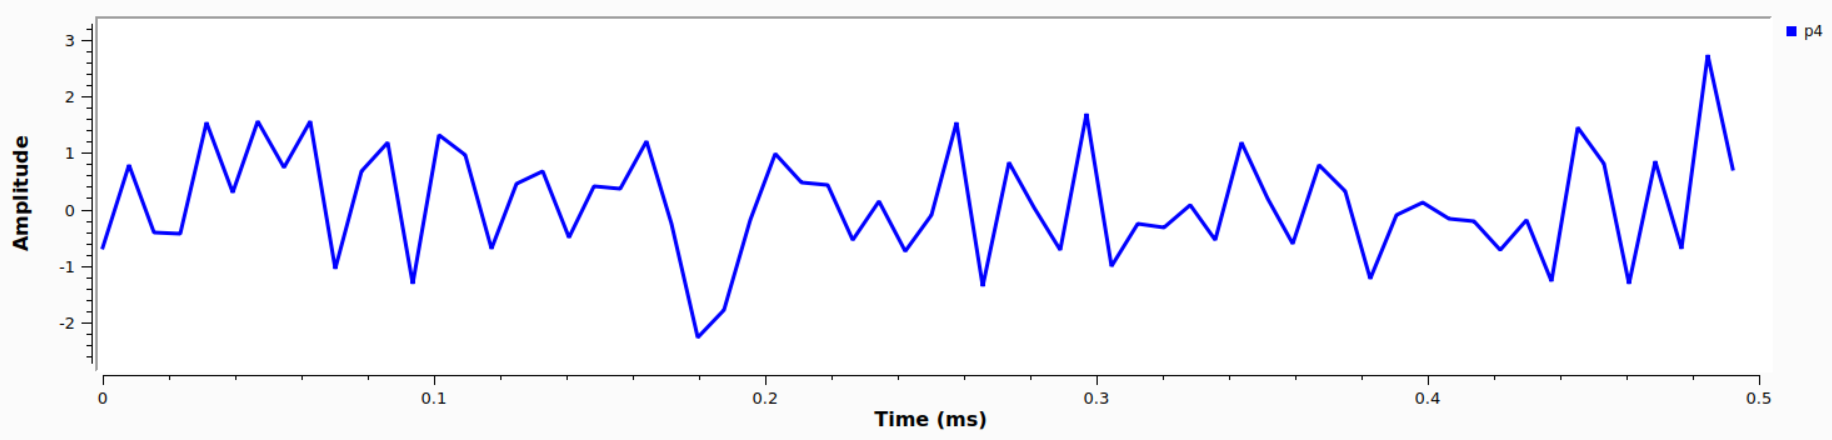
\includegraphics[width=\textwidth]{imagenes/ruido_puro_tiempo.png} 
    \caption{Ruido blanco en el dominio del tiempo.}
    \label{fig:ruido_tiempo}
\end{subfigure}
\hfill
\begin{subfigure}[b]{0.45\textwidth}
    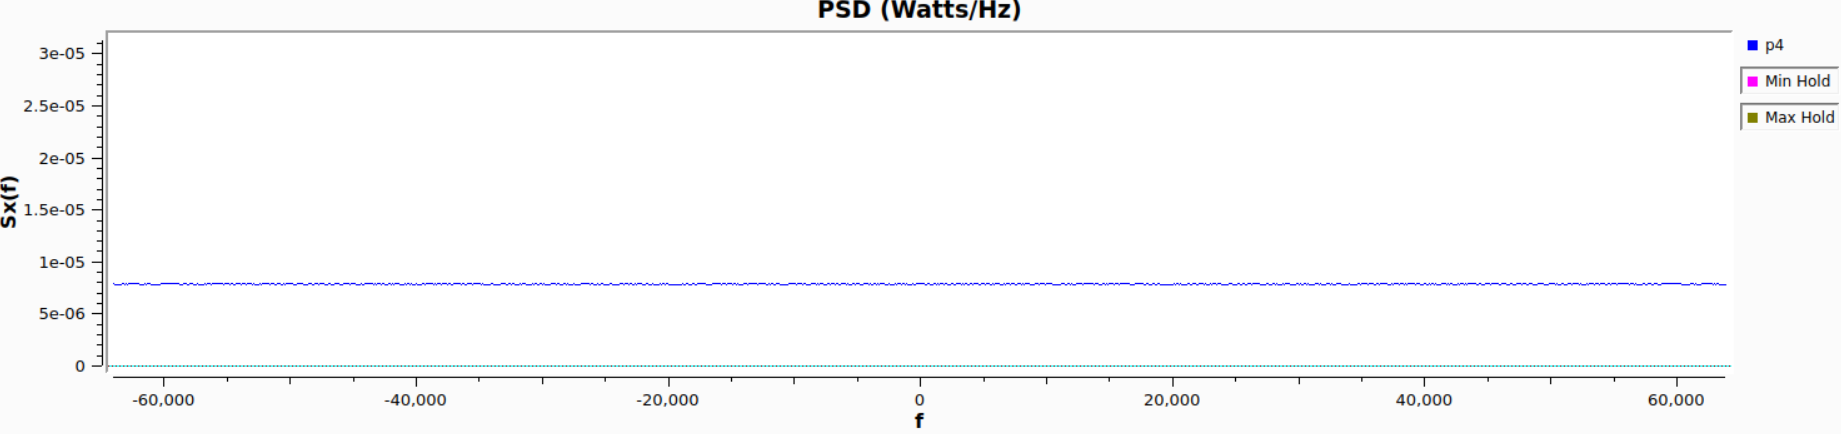
\includegraphics[width=\textwidth]{imagenes/ruido_puro_psd.png} 
    \caption{PSD del ruido blanco (Espectro plano).}
    \label{fig:ruido_psd}
\end{subfigure}
\caption{Análisis del ruido blanco gaussiano puro en los analizadores de GNU Radio.}
\label{fig:analisis_ruido_puro}
\end{figure}

\begin{figure}[htbp]
\centering
\begin{subfigure}[b]{0.45\textwidth}
    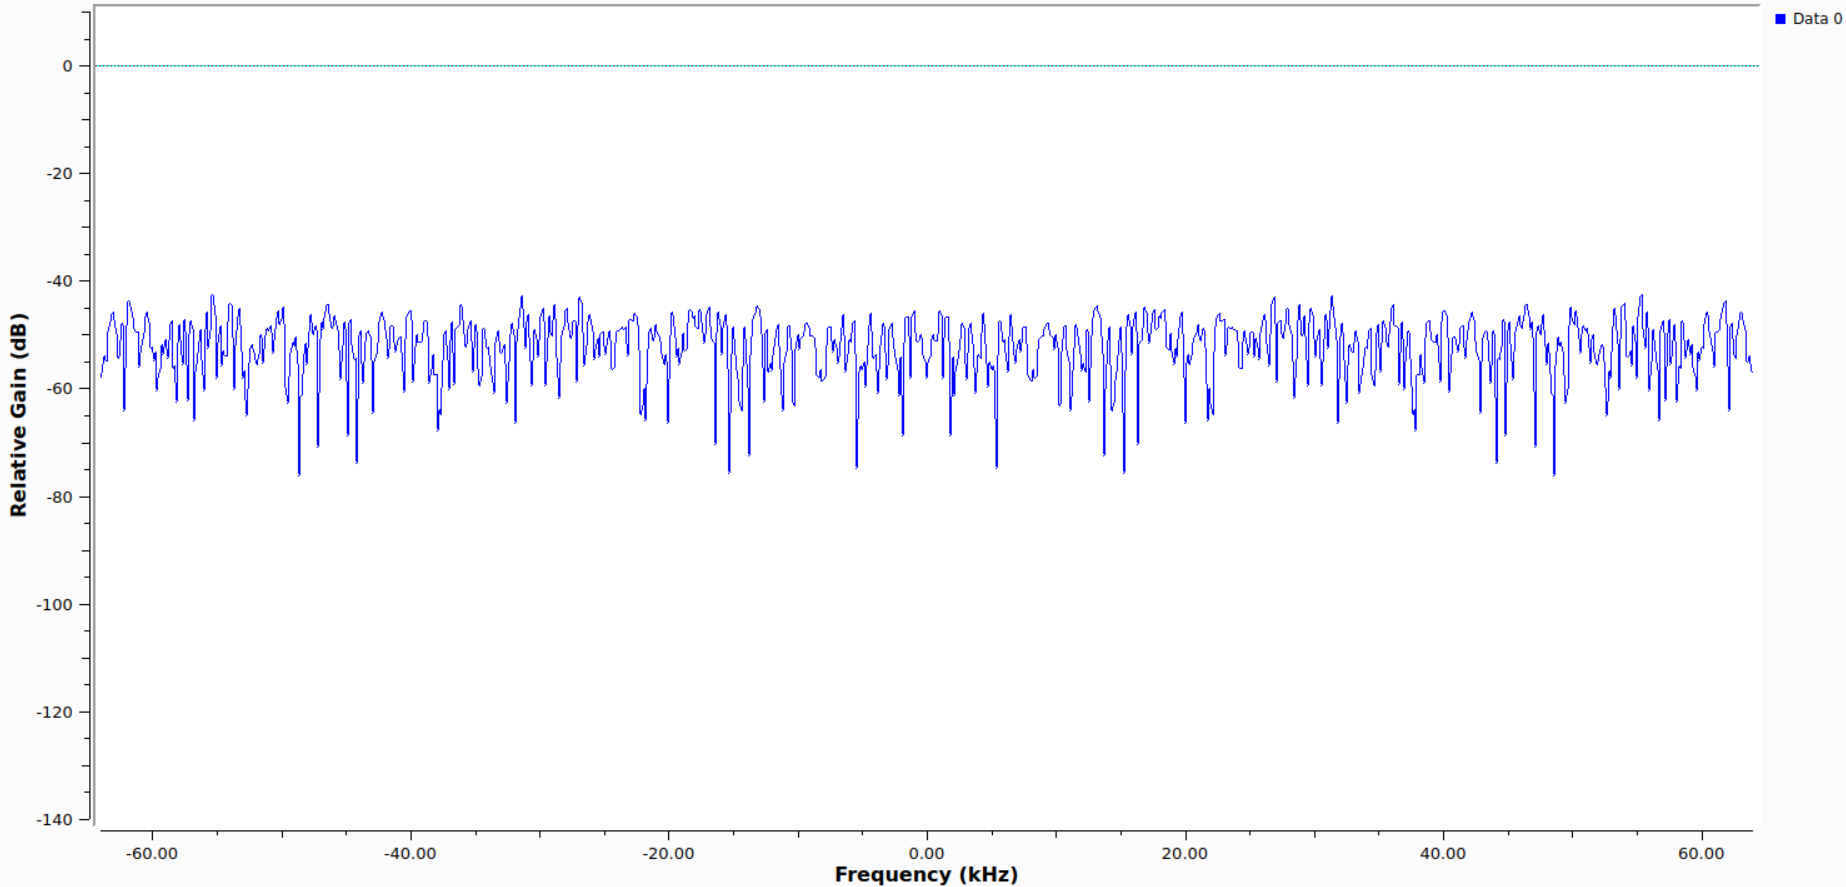
\includegraphics[width=\textwidth]{imagenes/espectro_amp_1.png} 
    \caption{espectro en frecuencia de ruido con amplitud de 1.}
    \label{fig:espectro_frecuencia_ruido_amp_1}
\end{subfigure}
\hfill
\begin{subfigure}[b]{0.45\textwidth}
    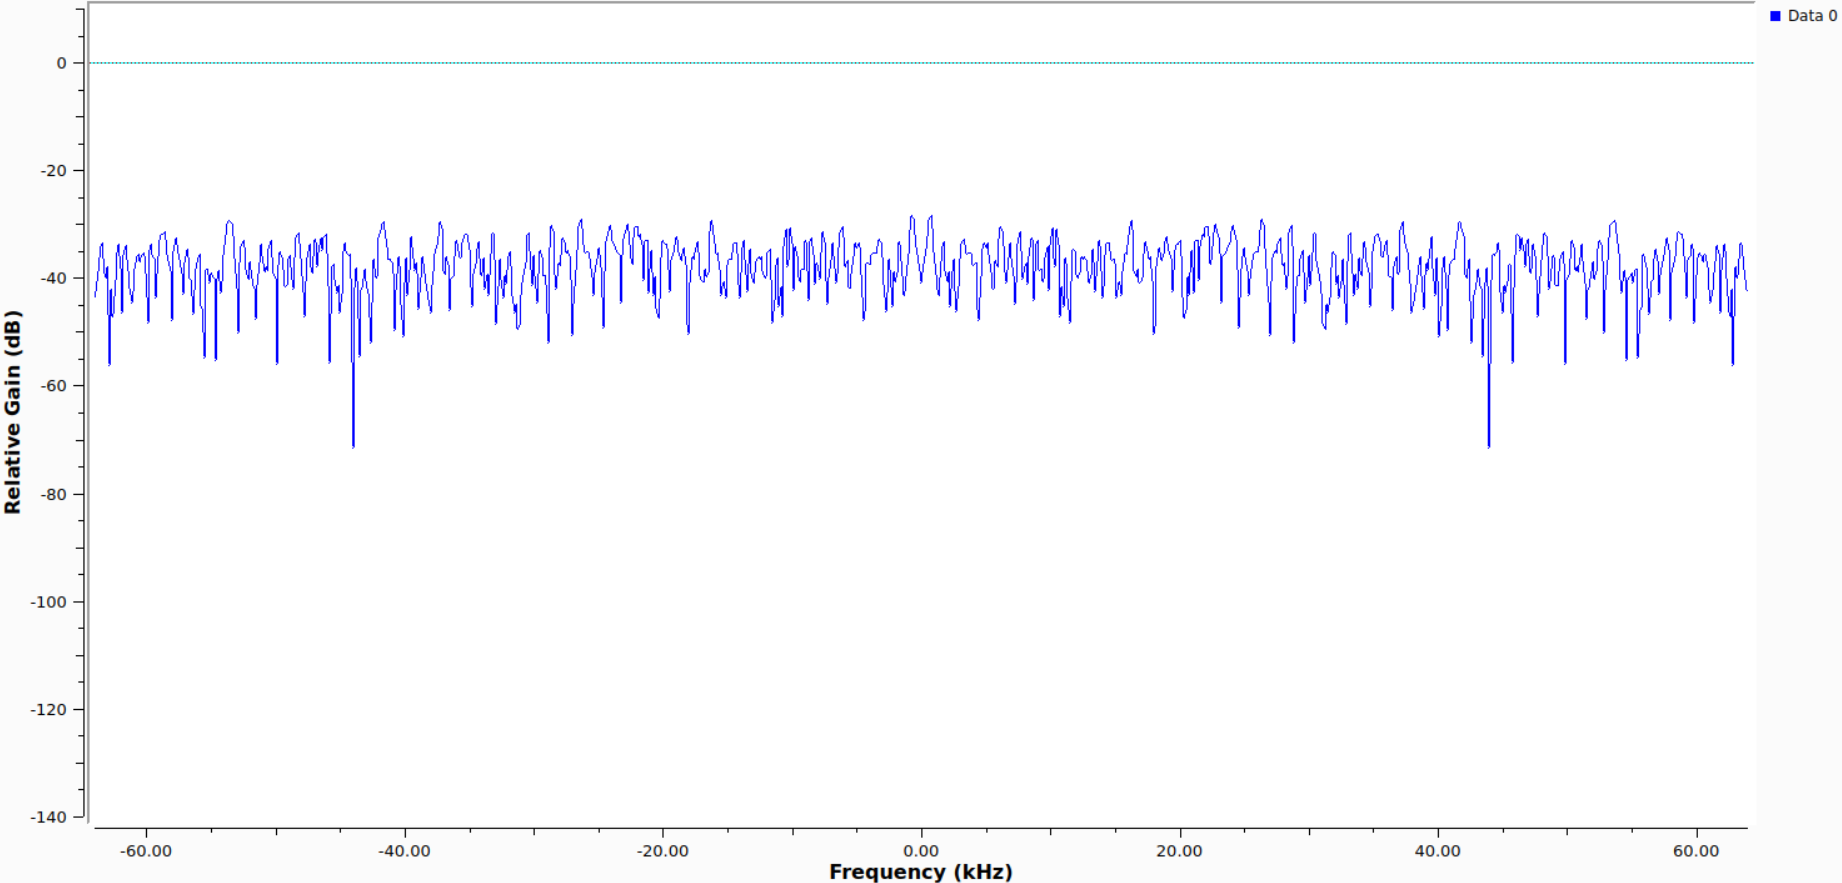
\includegraphics[width=\textwidth]{imagenes/espectro_amp_2.png} 
    \caption{espectro en frecuencia de ruido con amplitud de 0.2.}
    \label{fig:espectro_frecuencia_ruido_amp_0.2}
\end{subfigure}
\caption{cambio del nivel de potencia del ruido al variar la amplitud en el bloque generador.}
\label{fig:espectro_frecuencia_ruido}
\end{figure}
% --- FIN DEL MÓDULO ---